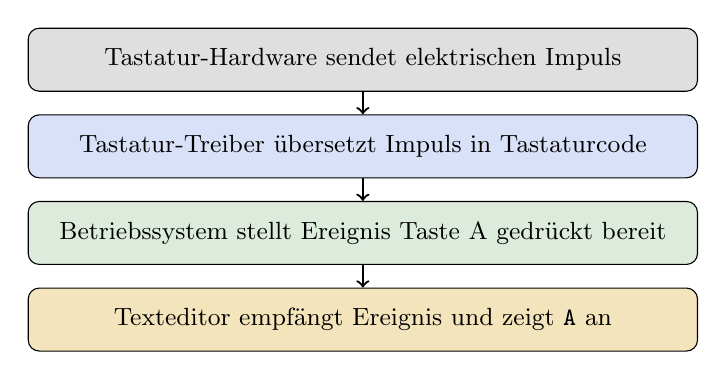
\begin{tikzpicture}[
    stepc/.style={draw, rounded corners, fill=RoyalBlue!15, minimum width=8.5cm, minimum height=0.8cm, text centered, font=\small},
    arrow/.style={->, thick}
]
    \node[stepc, fill=Gray!25]          (hw)  at (0, 3.3) {Tastatur-Hardware sendet elektrischen Impuls};
    \node[stepc, fill=RoyalBlue!20]     (drv) at (0, 2.2) {Tastatur-Treiber übersetzt Impuls in Tastaturcode};
    \node[stepc, fill=DarkSeaGreen!30]  (os)  at (0, 1.1) {Betriebssystem stellt Ereignis \enquote{Taste A gedrückt} bereit};
    \node[stepc, fill=Goldenrod!30]     (app) at (0, 0.0) {Texteditor empfängt Ereignis und zeigt \texttt{A} an};

    \draw[arrow] (hw)  -- (drv);
    \draw[arrow] (drv) -- (os);
    \draw[arrow] (os)  -- (app);
\end{tikzpicture}
